% !Mode:: "TeX:UTF-8"%確保文檔utf-8編碼
\documentclass[border=2pt]{standalone}
\usepackage{tikz}
\usepackage{pgfplots}
\pgfplotsset{compat=newest}
\usetikzlibrary{intersections,calc,positioning,backgrounds}


\begin{document}

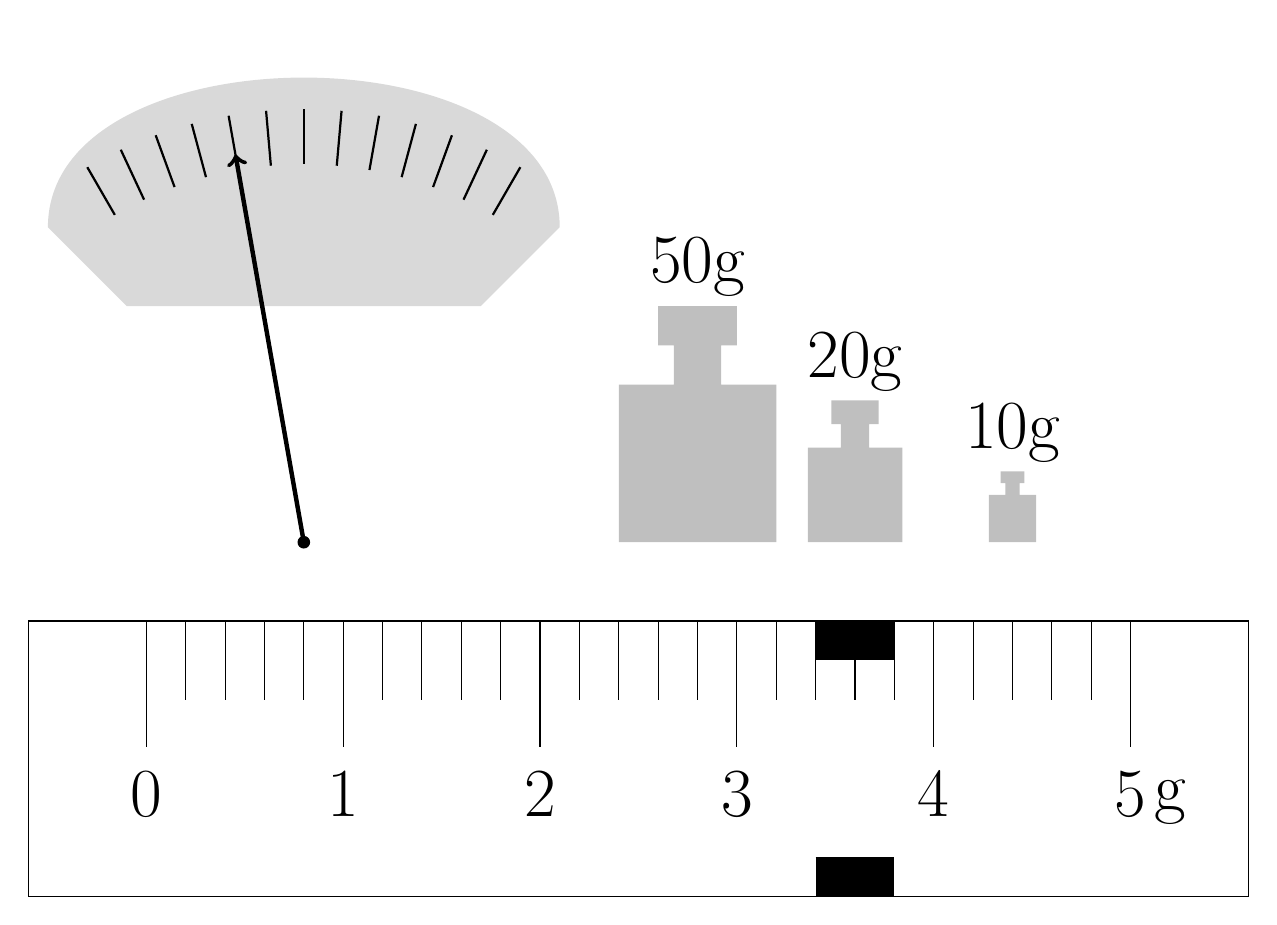
\begin{tikzpicture}


%刻度尺
\begin{scope}[xscale=0.5]

%显示的数值多少g
\def\gnum{3.4}
\pgfmathsetmacro{\gmove}{10*\gnum/2}
%主线轴
\def\startx{0}
\def\endx{25}
\pgfmathsetmacro{\stepx}{\startx+1}
\pgfmathsetmacro{\stepxfive}{\startx+5}
\pgfmathsetmacro{\stepxten}{\startx+10}

\coordinate (startpoint) at (\startx,0) ;
\coordinate (endpoint) at (\endx,0) ;
\draw [](startpoint) -- (endpoint);

\draw ($(startpoint) + (-3,-3.5)$) rectangle ($(endpoint) + (3,0)$);

%细小刻度
\foreach \x in {\startx,\stepx,...,\endx}
  \draw [](\x,0) -- (\x,-1);   

%5分之一刻度
%\foreach \y in {\startx,\stepxfive,...,\endx}
%  \draw [] (\y,-1.6) -- (\y,0);


%10分之一刻度
\foreach \i in {\startx,\stepxfive,...,\endx}
  \draw [] (\i,-1.6) -- (\i,0)
  node[below=1.8cm] {\Huge \pgfmathprint{int(\i/5)}};

%unit
\node at ($(endpoint) +(1,-2.3)$) {\Huge  g};


%额外的修改
\draw[line width =0.5cm,yshift=-0.25cm] (\gmove,0)-- +(2,0);
\begin{scope}[yshift=-3cm]
\draw[line width =0.5cm,yshift=-0.25cm] (\gmove,0)-- +(2,0);
\end{scope}

\end{scope}

%刻度尺之外的修改

%简单非定量表盘


\begin{scope}[xshift=2cm,yshift=1cm]
\fill (0,0) circle (0.08);
\fill[gray!30] (2.25,3) -- ++(1,1)  to[out=90,in=90]  ++(-6.5,0) -- +(1,-1);
\foreach \x in {60,65,...,120} \draw[thick] (\x:5.5) -- (\x:4.8);
\draw[ultra thick,->] (0,0) -- ++(100:5);
\end{scope}



%砝码1
\begin{scope}[xshift=7cm,yshift=1cm]
\fill[gray!50] (0,0) -- (1,0) -- (1,2) -- (0.3,2) -- (0.3,2.5) -- (0.5,2.5) -- (0.5,3)--(0,3) -- (-0.5,3)  -- (-0.5,2.5) -- (-0.3,2.5) -- (-0.3,2) -- (-1,2) -- (-1,0) --cycle;
\coordinate (weight-top) at (0,3);

\node [above =0cm of weight-top]{\Huge 50g};
\end{scope}

%砝码2
\begin{scope}[xshift=9cm,yshift=1cm]
\begin{scope}[scale=0.6]
\fill[gray!50] (0,0) -- (1,0) -- (1,2) -- (0.3,2) -- (0.3,2.5) -- (0.5,2.5) -- (0.5,3)--(0,3) -- (-0.5,3)  -- (-0.5,2.5) -- (-0.3,2.5) -- (-0.3,2) -- (-1,2) -- (-1,0) --cycle;
\coordinate (weight-top) at (0,3);
\end{scope}
\node [above =0cm of weight-top]{\Huge 20g};
\end{scope}

%砝码3
\begin{scope}[xshift=11cm,yshift=1cm]
\begin{scope}[scale=0.3]
\fill[gray!50] (0,0) -- (1,0) -- (1,2) -- (0.3,2) -- (0.3,2.5) -- (0.5,2.5) -- (0.5,3)--(0,3) -- (-0.5,3)  -- (-0.5,2.5) -- (-0.3,2.5) -- (-0.3,2) -- (-1,2) -- (-1,0) --cycle;
\coordinate (weight-top) at (0,3);
\end{scope}
\node [above =0cm of weight-top]{\Huge 10g};
\end{scope}





%待测物体



\end{tikzpicture}


\end{document}